\documentclass[twoside]{book}

% Packages required by doxygen
\usepackage{fixltx2e}
\usepackage{calc}
\usepackage{doxygen}
\usepackage[export]{adjustbox} % also loads graphicx
\usepackage{graphicx}
\usepackage[utf8]{inputenc}
\usepackage{makeidx}
\usepackage{multicol}
\usepackage{multirow}
\PassOptionsToPackage{warn}{textcomp}
\usepackage{textcomp}
\usepackage[nointegrals]{wasysym}
\usepackage[table]{xcolor}

% Font selection
\usepackage[T1]{fontenc}
\usepackage[scaled=.90]{helvet}
\usepackage{courier}
\usepackage{amssymb}
\usepackage{sectsty}
\renewcommand{\familydefault}{\sfdefault}
\allsectionsfont{%
  \fontseries{bc}\selectfont%
  \color{darkgray}%
}
\renewcommand{\DoxyLabelFont}{%
  \fontseries{bc}\selectfont%
  \color{darkgray}%
}
\newcommand{\+}{\discretionary{\mbox{\scriptsize$\hookleftarrow$}}{}{}}

% Page & text layout
\usepackage{geometry}
\geometry{%
  a4paper,%
  top=2.5cm,%
  bottom=2.5cm,%
  left=2.5cm,%
  right=2.5cm%
}
\tolerance=750
\hfuzz=15pt
\hbadness=750
\setlength{\emergencystretch}{15pt}
\setlength{\parindent}{0cm}
\setlength{\parskip}{3ex plus 2ex minus 2ex}
\makeatletter
\renewcommand{\paragraph}{%
  \@startsection{paragraph}{4}{0ex}{-1.0ex}{1.0ex}{%
    \normalfont\normalsize\bfseries\SS@parafont%
  }%
}
\renewcommand{\subparagraph}{%
  \@startsection{subparagraph}{5}{0ex}{-1.0ex}{1.0ex}{%
    \normalfont\normalsize\bfseries\SS@subparafont%
  }%
}
\makeatother

% Headers & footers
\usepackage{fancyhdr}
\pagestyle{fancyplain}
\fancyhead[LE]{\fancyplain{}{\bfseries\thepage}}
\fancyhead[CE]{\fancyplain{}{}}
\fancyhead[RE]{\fancyplain{}{\bfseries\leftmark}}
\fancyhead[LO]{\fancyplain{}{\bfseries\rightmark}}
\fancyhead[CO]{\fancyplain{}{}}
\fancyhead[RO]{\fancyplain{}{\bfseries\thepage}}
\fancyfoot[LE]{\fancyplain{}{}}
\fancyfoot[CE]{\fancyplain{}{}}
\fancyfoot[RE]{\fancyplain{}{\bfseries\scriptsize Generated by Doxygen }}
\fancyfoot[LO]{\fancyplain{}{\bfseries\scriptsize Generated by Doxygen }}
\fancyfoot[CO]{\fancyplain{}{}}
\fancyfoot[RO]{\fancyplain{}{}}
\renewcommand{\footrulewidth}{0.4pt}
\renewcommand{\chaptermark}[1]{%
  \markboth{#1}{}%
}
\renewcommand{\sectionmark}[1]{%
  \markright{\thesection\ #1}%
}

% Indices & bibliography
\usepackage{natbib}
\usepackage[titles]{tocloft}
\setcounter{tocdepth}{3}
\setcounter{secnumdepth}{5}
\makeindex

% Hyperlinks (required, but should be loaded last)
\usepackage{ifpdf}
\ifpdf
  \usepackage[pdftex,pagebackref=true]{hyperref}
\else
  \usepackage[ps2pdf,pagebackref=true]{hyperref}
\fi
\hypersetup{%
  colorlinks=true,%
  linkcolor=blue,%
  citecolor=blue,%
  unicode%
}

% Custom commands
\newcommand{\clearemptydoublepage}{%
  \newpage{\pagestyle{empty}\cleardoublepage}%
}

\usepackage{caption}
\captionsetup{labelsep=space,justification=centering,font={bf},singlelinecheck=off,skip=4pt,position=top}

%===== C O N T E N T S =====

\begin{document}

% Titlepage & ToC
\hypersetup{pageanchor=false,
             bookmarksnumbered=true,
             pdfencoding=unicode
            }
\pagenumbering{alph}
\begin{titlepage}
\vspace*{7cm}
\begin{center}%
{\Large My Project }\\
\vspace*{1cm}
{\large Generated by Doxygen 1.8.14}\\
\end{center}
\end{titlepage}
\clearemptydoublepage
\pagenumbering{roman}
\tableofcontents
\clearemptydoublepage
\pagenumbering{arabic}
\hypersetup{pageanchor=true}

%--- Begin generated contents ---
\chapter{Hierarchical Index}
\section{Class Hierarchy}
This inheritance list is sorted roughly, but not completely, alphabetically\+:\begin{DoxyCompactList}
\item exception\begin{DoxyCompactList}
\item \contentsline{section}{exc\+\_\+argument}{\pageref{classexc__argument}}{}
\item \contentsline{section}{plikb}{\pageref{classplikb}}{}
\end{DoxyCompactList}
\item \contentsline{section}{Kolekcja}{\pageref{class_kolekcja}}{}
\item \contentsline{section}{Produkty}{\pageref{class_produkty}}{}
\begin{DoxyCompactList}
\item \contentsline{section}{Narzedzia}{\pageref{class_narzedzia}}{}
\item \contentsline{section}{Skrzynki}{\pageref{class_skrzynki}}{}
\begin{DoxyCompactList}
\item \contentsline{section}{Skrzynka\+\_\+z\+\_\+srubkami}{\pageref{class_skrzynka__z__srubkami}}{}
\end{DoxyCompactList}
\item \contentsline{section}{Srubki}{\pageref{class_srubki}}{}
\begin{DoxyCompactList}
\item \contentsline{section}{Skrzynka\+\_\+z\+\_\+srubkami}{\pageref{class_skrzynka__z__srubkami}}{}
\end{DoxyCompactList}
\end{DoxyCompactList}
\end{DoxyCompactList}

\chapter{Class Index}
\section{Class List}
Here are the classes, structs, unions and interfaces with brief descriptions\+:\begin{DoxyCompactList}
\item\contentsline{section}{\mbox{\hyperlink{classexc__argument}{exc\+\_\+argument}} }{\pageref{classexc__argument}}{}
\item\contentsline{section}{\mbox{\hyperlink{class_kolekcja}{Kolekcja}} }{\pageref{class_kolekcja}}{}
\item\contentsline{section}{\mbox{\hyperlink{class_narzedzia}{Narzedzia}} }{\pageref{class_narzedzia}}{}
\item\contentsline{section}{\mbox{\hyperlink{classplikb}{plikb}} }{\pageref{classplikb}}{}
\item\contentsline{section}{\mbox{\hyperlink{class_produkty}{Produkty}} }{\pageref{class_produkty}}{}
\item\contentsline{section}{\mbox{\hyperlink{class_skrzynka__z__srubkami}{Skrzynka\+\_\+z\+\_\+srubkami}} }{\pageref{class_skrzynka__z__srubkami}}{}
\item\contentsline{section}{\mbox{\hyperlink{class_skrzynki}{Skrzynki}} }{\pageref{class_skrzynki}}{}
\item\contentsline{section}{\mbox{\hyperlink{class_srubki}{Srubki}} }{\pageref{class_srubki}}{}
\end{DoxyCompactList}

\chapter{Class Documentation}
\hypertarget{classexc__argument}{}\section{exc\+\_\+argument Class Reference}
\label{classexc__argument}\index{exc\+\_\+argument@{exc\+\_\+argument}}


{\ttfamily \#include $<$Wyjatki.\+h$>$}

Inheritance diagram for exc\+\_\+argument\+:\begin{figure}[H]
\begin{center}
\leavevmode
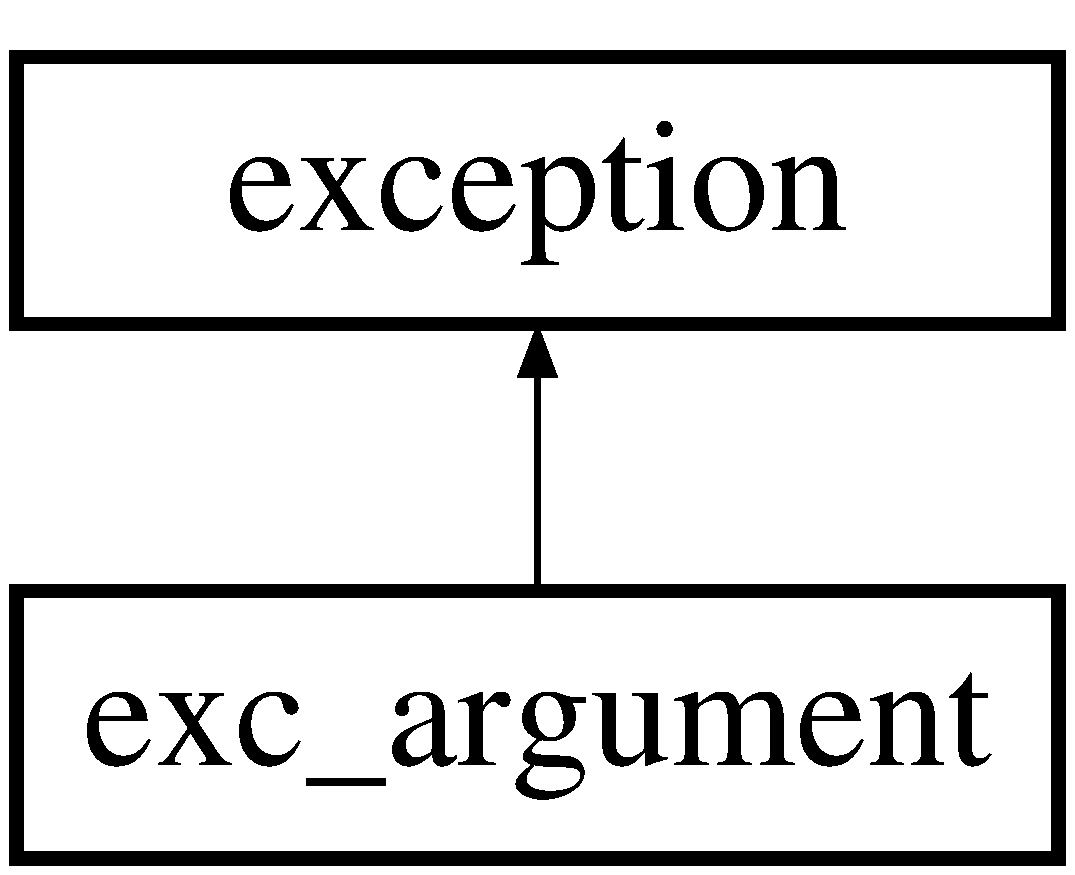
\includegraphics[height=2.000000cm]{classexc__argument}
\end{center}
\end{figure}
\subsection*{Public Member Functions}
\begin{DoxyCompactItemize}
\item 
\mbox{\Hypertarget{classexc__argument_a3e893e3da4e63c23a0709130bab2dd73}\label{classexc__argument_a3e893e3da4e63c23a0709130bab2dd73}} 
{\bfseries exc\+\_\+argument} (double arg=0)
\item 
virtual const char $\ast$ \mbox{\hyperlink{classexc__argument_a0b2a620ca9b3e2206fb8a8fe9e4c6c20}{what}} () const noexcept
\end{DoxyCompactItemize}


\subsection{Detailed Description}
Klasa wyjatkow dziedziczaca po klasie exception 

\subsection{Member Function Documentation}
\mbox{\Hypertarget{classexc__argument_a0b2a620ca9b3e2206fb8a8fe9e4c6c20}\label{classexc__argument_a0b2a620ca9b3e2206fb8a8fe9e4c6c20}} 
\index{exc\+\_\+argument@{exc\+\_\+argument}!what@{what}}
\index{what@{what}!exc\+\_\+argument@{exc\+\_\+argument}}
\subsubsection{\texorpdfstring{what()}{what()}}
{\footnotesize\ttfamily virtual const char$\ast$ exc\+\_\+argument\+::what (\begin{DoxyParamCaption}{ }\end{DoxyParamCaption}) const\hspace{0.3cm}{\ttfamily [inline]}, {\ttfamily [virtual]}, {\ttfamily [noexcept]}}

metoda uruchamiajaca sie po wrowadzeniu blednej wartosci 

The documentation for this class was generated from the following file\+:\begin{DoxyCompactItemize}
\item 
Wyjatki.\+h\end{DoxyCompactItemize}

\hypertarget{class_kolekcja}{}\section{Kolekcja Class Reference}
\label{class_kolekcja}\index{Kolekcja@{Kolekcja}}


{\ttfamily \#include $<$Kolekcja.\+h$>$}

\subsection*{Public Member Functions}
\begin{DoxyCompactItemize}
\item 
int \mbox{\hyperlink{class_kolekcja_ade81cbf8bb9e0251cd8cb217eca813e4}{Czy\+\_\+pusta}} ()
\item 
void \mbox{\hyperlink{class_kolekcja_a8631b63e89e8b0b4761aa888297e9f4a}{Dodaj}} (\mbox{\hyperlink{class_produkty}{Produkty}} \&z)
\item 
void \mbox{\hyperlink{class_kolekcja_af76172e2b430490eaea2b2f553a598a6}{Wypisz}} ()
\item 
void \mbox{\hyperlink{class_kolekcja_adb7f74fefe7f8713fbececd03a3740d0}{zapis}} ()
\end{DoxyCompactItemize}


\subsection{Detailed Description}
Klasa \mbox{\hyperlink{class_kolekcja}{Kolekcja}} umozliwia reprezentacje oraz wprowadzanie produktow do wspolnej kategorii 

\subsection{Member Function Documentation}
\mbox{\Hypertarget{class_kolekcja_ade81cbf8bb9e0251cd8cb217eca813e4}\label{class_kolekcja_ade81cbf8bb9e0251cd8cb217eca813e4}} 
\index{Kolekcja@{Kolekcja}!Czy\+\_\+pusta@{Czy\+\_\+pusta}}
\index{Czy\+\_\+pusta@{Czy\+\_\+pusta}!Kolekcja@{Kolekcja}}
\subsubsection{\texorpdfstring{Czy\+\_\+pusta()}{Czy\_pusta()}}
{\footnotesize\ttfamily int Kolekcja\+::\+Czy\+\_\+pusta (\begin{DoxyParamCaption}{ }\end{DoxyParamCaption})}

metoda sprawdzajaca czy lisa jest pusta \begin{DoxyReturn}{Returns}
-\/ 0 gdy pusta 1 gdy cos jest w liscie 
\end{DoxyReturn}
\mbox{\Hypertarget{class_kolekcja_a8631b63e89e8b0b4761aa888297e9f4a}\label{class_kolekcja_a8631b63e89e8b0b4761aa888297e9f4a}} 
\index{Kolekcja@{Kolekcja}!Dodaj@{Dodaj}}
\index{Dodaj@{Dodaj}!Kolekcja@{Kolekcja}}
\subsubsection{\texorpdfstring{Dodaj()}{Dodaj()}}
{\footnotesize\ttfamily void Kolekcja\+::\+Dodaj (\begin{DoxyParamCaption}\item[{\mbox{\hyperlink{class_produkty}{Produkty}} \&}]{z }\end{DoxyParamCaption})}

metoda dodajaca nowy element do danej kolekcji 
\begin{DoxyParams}{Parameters}
{\em -\/\+Nowy} & element klasy \mbox{\hyperlink{class_produkty}{Produkty}} \\
\hline
\end{DoxyParams}
\mbox{\Hypertarget{class_kolekcja_af76172e2b430490eaea2b2f553a598a6}\label{class_kolekcja_af76172e2b430490eaea2b2f553a598a6}} 
\index{Kolekcja@{Kolekcja}!Wypisz@{Wypisz}}
\index{Wypisz@{Wypisz}!Kolekcja@{Kolekcja}}
\subsubsection{\texorpdfstring{Wypisz()}{Wypisz()}}
{\footnotesize\ttfamily void Kolekcja\+::\+Wypisz (\begin{DoxyParamCaption}{ }\end{DoxyParamCaption})}

metoda wypisujaca dane poszczegulnych kolekcji \mbox{\Hypertarget{class_kolekcja_adb7f74fefe7f8713fbececd03a3740d0}\label{class_kolekcja_adb7f74fefe7f8713fbececd03a3740d0}} 
\index{Kolekcja@{Kolekcja}!zapis@{zapis}}
\index{zapis@{zapis}!Kolekcja@{Kolekcja}}
\subsubsection{\texorpdfstring{zapis()}{zapis()}}
{\footnotesize\ttfamily void Kolekcja\+::zapis (\begin{DoxyParamCaption}{ }\end{DoxyParamCaption})}

metoda sluzaca do zapisu do pliku danych z listy produktow 

The documentation for this class was generated from the following files\+:\begin{DoxyCompactItemize}
\item 
Kolekcja.\+h\item 
Kolekcja.\+cpp\end{DoxyCompactItemize}

\hypertarget{class_narzedzia}{}\section{Narzedzia Class Reference}
\label{class_narzedzia}\index{Narzedzia@{Narzedzia}}


{\ttfamily \#include $<$Narzedzia.\+h$>$}

Inheritance diagram for Narzedzia\+:\begin{figure}[H]
\begin{center}
\leavevmode
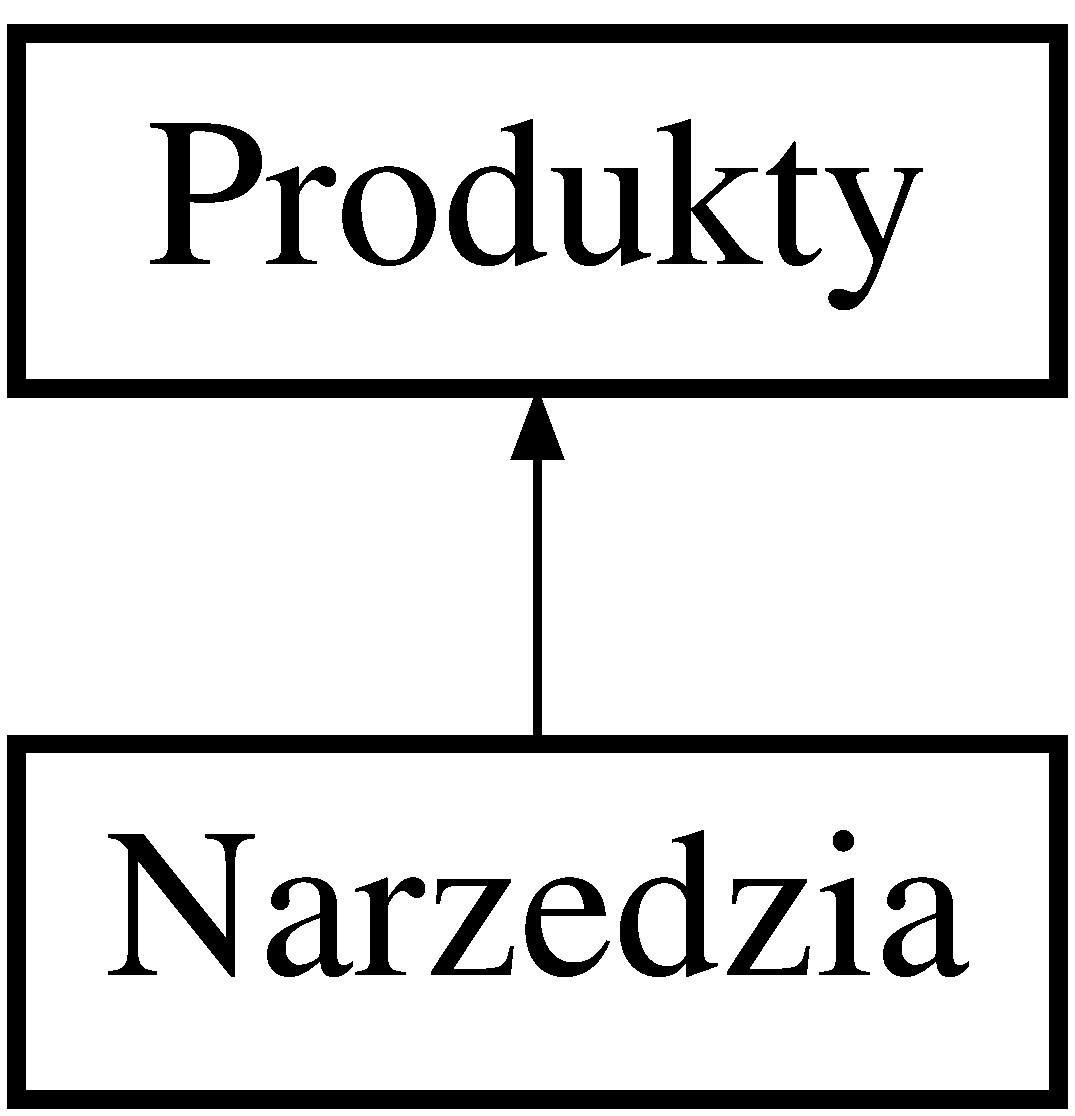
\includegraphics[height=2.000000cm]{class_narzedzia}
\end{center}
\end{figure}
\subsection*{Public Member Functions}
\begin{DoxyCompactItemize}
\item 
void \mbox{\hyperlink{class_narzedzia_ade1bd4ecf05c894b263791bfcf0f876f}{wstaw}} ()
\item 
void \mbox{\hyperlink{class_narzedzia_a39cd48d9367f3a4e8fcc30878a320338}{wypisz}} ()
\item 
void \mbox{\hyperlink{class_narzedzia_a4178a26508e00853e8c5c483f9a439a3}{zapisz}} (std\+::ostream \&o) const
\end{DoxyCompactItemize}
\subsection*{Additional Inherited Members}


\subsection{Detailed Description}
Klasa pochodna klasy produkty reprezentuje dane o narzedziach 

\subsection{Member Function Documentation}
\mbox{\Hypertarget{class_narzedzia_ade1bd4ecf05c894b263791bfcf0f876f}\label{class_narzedzia_ade1bd4ecf05c894b263791bfcf0f876f}} 
\index{Narzedzia@{Narzedzia}!wstaw@{wstaw}}
\index{wstaw@{wstaw}!Narzedzia@{Narzedzia}}
\subsubsection{\texorpdfstring{wstaw()}{wstaw()}}
{\footnotesize\ttfamily void Narzedzia\+::wstaw (\begin{DoxyParamCaption}{ }\end{DoxyParamCaption})\hspace{0.3cm}{\ttfamily [virtual]}}

metoda sluzaca do wprowadzanaia danych charakteryzujacych narzedzia z klawiatury 

Reimplemented from \mbox{\hyperlink{class_produkty_ad69fa64c8984c55fe9b1a2ade607a0ed}{Produkty}}.

\mbox{\Hypertarget{class_narzedzia_a39cd48d9367f3a4e8fcc30878a320338}\label{class_narzedzia_a39cd48d9367f3a4e8fcc30878a320338}} 
\index{Narzedzia@{Narzedzia}!wypisz@{wypisz}}
\index{wypisz@{wypisz}!Narzedzia@{Narzedzia}}
\subsubsection{\texorpdfstring{wypisz()}{wypisz()}}
{\footnotesize\ttfamily void Narzedzia\+::wypisz (\begin{DoxyParamCaption}{ }\end{DoxyParamCaption})\hspace{0.3cm}{\ttfamily [virtual]}}

metoda sluzaca do wypisywania danych charakteryzujacych narzedzia z klawiatury 

Reimplemented from \mbox{\hyperlink{class_produkty_a720c6591cfbb332f99baccf0f54c4ada}{Produkty}}.

\mbox{\Hypertarget{class_narzedzia_a4178a26508e00853e8c5c483f9a439a3}\label{class_narzedzia_a4178a26508e00853e8c5c483f9a439a3}} 
\index{Narzedzia@{Narzedzia}!zapisz@{zapisz}}
\index{zapisz@{zapisz}!Narzedzia@{Narzedzia}}
\subsubsection{\texorpdfstring{zapisz()}{zapisz()}}
{\footnotesize\ttfamily void Narzedzia\+::zapisz (\begin{DoxyParamCaption}\item[{std\+::ostream \&}]{o }\end{DoxyParamCaption}) const\hspace{0.3cm}{\ttfamily [virtual]}}

metoda zapisujaca dane o narzedziach do pliku wprowadzane podczas dzialania programu 

Reimplemented from \mbox{\hyperlink{class_produkty_a49c2ba4084346df8e7c987b9ec62676e}{Produkty}}.



The documentation for this class was generated from the following files\+:\begin{DoxyCompactItemize}
\item 
Narzedzia.\+h\item 
Narzedzia.\+cpp\end{DoxyCompactItemize}

\hypertarget{classplikb}{}\section{plikb Class Reference}
\label{classplikb}\index{plikb@{plikb}}


{\ttfamily \#include $<$Wyjatki.\+h$>$}

Inheritance diagram for plikb\+:\begin{figure}[H]
\begin{center}
\leavevmode
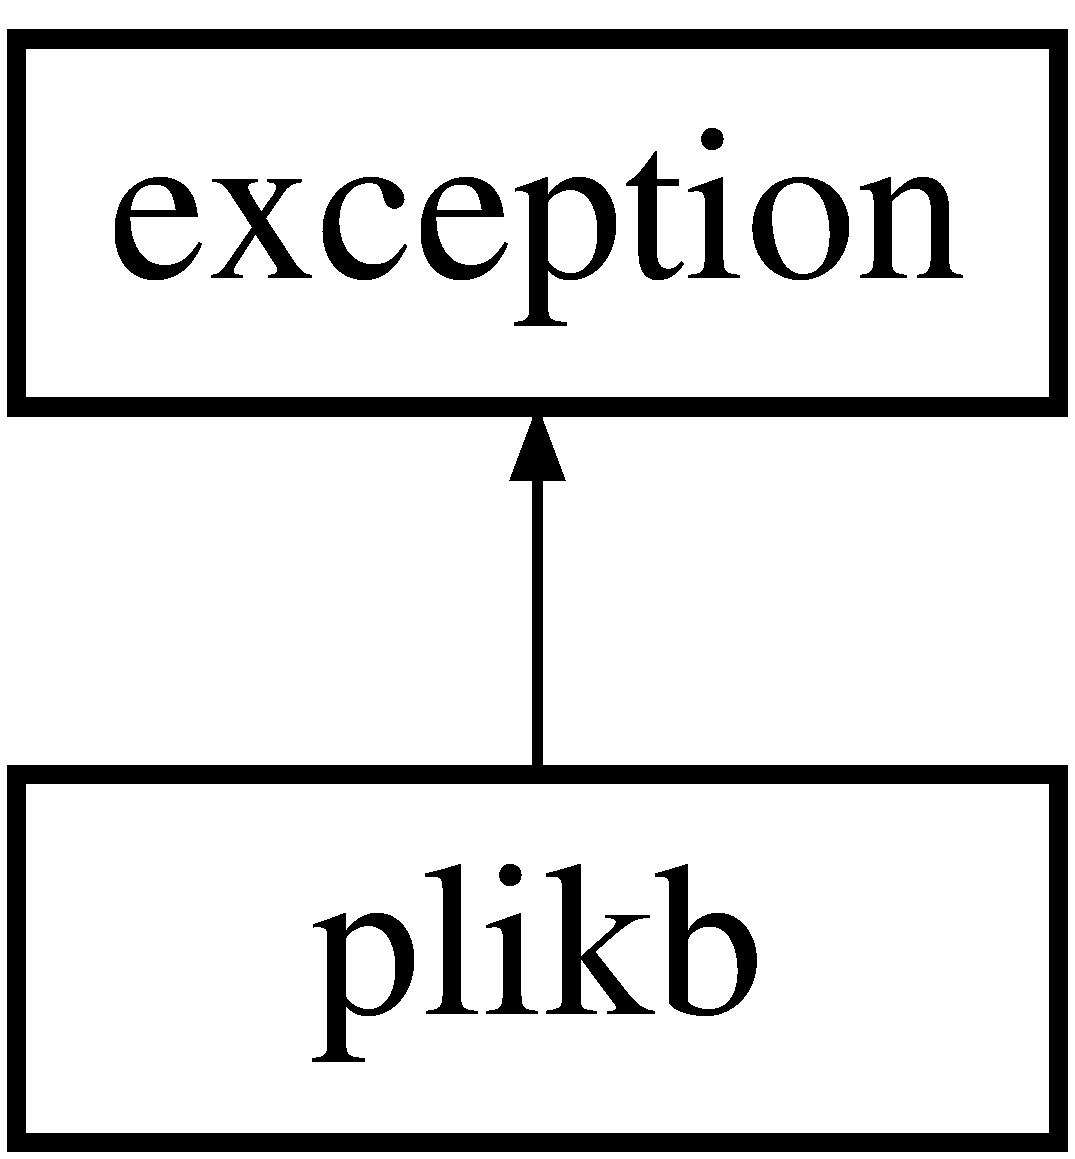
\includegraphics[height=2.000000cm]{classplikb}
\end{center}
\end{figure}
\subsection*{Public Member Functions}
\begin{DoxyCompactItemize}
\item 
\mbox{\Hypertarget{classplikb_a03dadb3945ee571ce073806d0f252931}\label{classplikb_a03dadb3945ee571ce073806d0f252931}} 
{\bfseries plikb} (string tmp)
\item 
const char $\ast$ \mbox{\hyperlink{classplikb_a99be76b11eb582db85d825b3bbf1da8e}{what}} (void) const noexcept override
\end{DoxyCompactItemize}


\subsection{Detailed Description}
Klasa wyjatkow dziedziczaca po klasie exception dla plikow 

\subsection{Member Function Documentation}
\mbox{\Hypertarget{classplikb_a99be76b11eb582db85d825b3bbf1da8e}\label{classplikb_a99be76b11eb582db85d825b3bbf1da8e}} 
\index{plikb@{plikb}!what@{what}}
\index{what@{what}!plikb@{plikb}}
\subsubsection{\texorpdfstring{what()}{what()}}
{\footnotesize\ttfamily const char$\ast$ plikb\+::what (\begin{DoxyParamCaption}\item[{void}]{ }\end{DoxyParamCaption}) const\hspace{0.3cm}{\ttfamily [inline]}, {\ttfamily [override]}, {\ttfamily [noexcept]}}

metoda uruchamiajaca sie gdy plik jest bledy 

The documentation for this class was generated from the following file\+:\begin{DoxyCompactItemize}
\item 
Wyjatki.\+h\end{DoxyCompactItemize}

\hypertarget{class_produkty}{}\section{Produkty Class Reference}
\label{class_produkty}\index{Produkty@{Produkty}}


{\ttfamily \#include $<$Produkty.\+h$>$}

Inheritance diagram for Produkty\+:\begin{figure}[H]
\begin{center}
\leavevmode
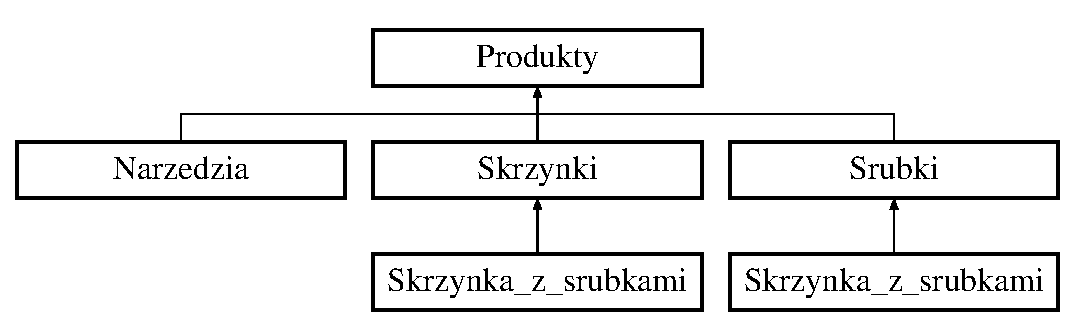
\includegraphics[height=3.000000cm]{class_produkty}
\end{center}
\end{figure}
\subsection*{Public Member Functions}
\begin{DoxyCompactItemize}
\item 
virtual void \mbox{\hyperlink{class_produkty_a720c6591cfbb332f99baccf0f54c4ada}{wypisz}} ()
\item 
void \mbox{\hyperlink{class_produkty_a73fe67e794f741b972330c09a8cf8e55}{Wstaw\+\_\+nazwe\+\_\+cene}} ()
\item 
void \mbox{\hyperlink{class_produkty_ac38af686bb465b62fd499dec9dd6c246}{Wypisz\+\_\+nazwe\+\_\+cene}} ()
\end{DoxyCompactItemize}
\subsection*{Protected Member Functions}
\begin{DoxyCompactItemize}
\item 
virtual void \mbox{\hyperlink{class_produkty_ad69fa64c8984c55fe9b1a2ade607a0ed}{wstaw}} ()
\item 
virtual void \mbox{\hyperlink{class_produkty_a49c2ba4084346df8e7c987b9ec62676e}{zapisz}} (std\+::ostream \&o) const
\end{DoxyCompactItemize}
\subsection*{Protected Attributes}
\begin{DoxyCompactItemize}
\item 
\mbox{\Hypertarget{class_produkty_aafbfed7251061470ba934e02ef902428}\label{class_produkty_aafbfed7251061470ba934e02ef902428}} 
string {\bfseries nazwa}
\item 
\mbox{\Hypertarget{class_produkty_a28eb276dae9d80062d5384be339d87d9}\label{class_produkty_a28eb276dae9d80062d5384be339d87d9}} 
float {\bfseries cena}
\end{DoxyCompactItemize}
\subsection*{Friends}
\begin{DoxyCompactItemize}
\item 
std\+::ostream \& \mbox{\hyperlink{class_produkty_a222d7f697f1aa66b79aefe7163945973}{operator$<$$<$}} (std\+::ostream \&o, \mbox{\hyperlink{class_produkty}{Produkty}} \&p)
\end{DoxyCompactItemize}


\subsection{Detailed Description}
Klasa abstrakcyjna \mbox{\hyperlink{class_produkty}{Produkty}} umozliwiajaca wprowadzanie oraz reprezentacjie czesci danych o nowych produktach 

\subsection{Member Function Documentation}
\mbox{\Hypertarget{class_produkty_ad69fa64c8984c55fe9b1a2ade607a0ed}\label{class_produkty_ad69fa64c8984c55fe9b1a2ade607a0ed}} 
\index{Produkty@{Produkty}!wstaw@{wstaw}}
\index{wstaw@{wstaw}!Produkty@{Produkty}}
\subsubsection{\texorpdfstring{wstaw()}{wstaw()}}
{\footnotesize\ttfamily void Produkty\+::wstaw (\begin{DoxyParamCaption}{ }\end{DoxyParamCaption})\hspace{0.3cm}{\ttfamily [protected]}, {\ttfamily [virtual]}}

metoda wirtualna sluzaca do wprowadzanaia danych z klawiatury 

Reimplemented in \mbox{\hyperlink{class_skrzynki_a764d5064b25a294b3309dc5077a77921}{Skrzynki}}, \mbox{\hyperlink{class_srubki_a129b7fcf23ad1928f196ca255aa66438}{Srubki}}, \mbox{\hyperlink{class_narzedzia_ade1bd4ecf05c894b263791bfcf0f876f}{Narzedzia}}, and \mbox{\hyperlink{class_skrzynka__z__srubkami_a4726c1844080cb96e833cf16e977ecb3}{Skrzynka\+\_\+z\+\_\+srubkami}}.

\mbox{\Hypertarget{class_produkty_a73fe67e794f741b972330c09a8cf8e55}\label{class_produkty_a73fe67e794f741b972330c09a8cf8e55}} 
\index{Produkty@{Produkty}!Wstaw\+\_\+nazwe\+\_\+cene@{Wstaw\+\_\+nazwe\+\_\+cene}}
\index{Wstaw\+\_\+nazwe\+\_\+cene@{Wstaw\+\_\+nazwe\+\_\+cene}!Produkty@{Produkty}}
\subsubsection{\texorpdfstring{Wstaw\+\_\+nazwe\+\_\+cene()}{Wstaw\_nazwe\_cene()}}
{\footnotesize\ttfamily void Produkty\+::\+Wstaw\+\_\+nazwe\+\_\+cene (\begin{DoxyParamCaption}{ }\end{DoxyParamCaption})}

metoda umozliwiajaca wprowadzenie danych o nazwie i cenie \mbox{\Hypertarget{class_produkty_a720c6591cfbb332f99baccf0f54c4ada}\label{class_produkty_a720c6591cfbb332f99baccf0f54c4ada}} 
\index{Produkty@{Produkty}!wypisz@{wypisz}}
\index{wypisz@{wypisz}!Produkty@{Produkty}}
\subsubsection{\texorpdfstring{wypisz()}{wypisz()}}
{\footnotesize\ttfamily void Produkty\+::wypisz (\begin{DoxyParamCaption}{ }\end{DoxyParamCaption})\hspace{0.3cm}{\ttfamily [virtual]}}

metoda wirtualna wypisujaca dane 

Reimplemented in \mbox{\hyperlink{class_skrzynki_adcf60a88ed78fba5a2dfdb54fa82b236}{Skrzynki}}, \mbox{\hyperlink{class_srubki_a0ac1f1ce5748283a13b0f554add73f0b}{Srubki}}, \mbox{\hyperlink{class_narzedzia_a39cd48d9367f3a4e8fcc30878a320338}{Narzedzia}}, and \mbox{\hyperlink{class_skrzynka__z__srubkami_ac543a438ce88bc79a9e8a398b6beff7c}{Skrzynka\+\_\+z\+\_\+srubkami}}.

\mbox{\Hypertarget{class_produkty_ac38af686bb465b62fd499dec9dd6c246}\label{class_produkty_ac38af686bb465b62fd499dec9dd6c246}} 
\index{Produkty@{Produkty}!Wypisz\+\_\+nazwe\+\_\+cene@{Wypisz\+\_\+nazwe\+\_\+cene}}
\index{Wypisz\+\_\+nazwe\+\_\+cene@{Wypisz\+\_\+nazwe\+\_\+cene}!Produkty@{Produkty}}
\subsubsection{\texorpdfstring{Wypisz\+\_\+nazwe\+\_\+cene()}{Wypisz\_nazwe\_cene()}}
{\footnotesize\ttfamily void Produkty\+::\+Wypisz\+\_\+nazwe\+\_\+cene (\begin{DoxyParamCaption}{ }\end{DoxyParamCaption})}

metoda wypisujaca dane o nazwie i cenie \mbox{\Hypertarget{class_produkty_a49c2ba4084346df8e7c987b9ec62676e}\label{class_produkty_a49c2ba4084346df8e7c987b9ec62676e}} 
\index{Produkty@{Produkty}!zapisz@{zapisz}}
\index{zapisz@{zapisz}!Produkty@{Produkty}}
\subsubsection{\texorpdfstring{zapisz()}{zapisz()}}
{\footnotesize\ttfamily void Produkty\+::zapisz (\begin{DoxyParamCaption}\item[{std\+::ostream \&}]{o }\end{DoxyParamCaption}) const\hspace{0.3cm}{\ttfamily [protected]}, {\ttfamily [virtual]}}

metoda zapisujaca dane do pliku wprowadzane podczas dzialania programu 

Reimplemented in \mbox{\hyperlink{class_skrzynki_a2980647e51a17161872064efc5f1b185}{Skrzynki}}, \mbox{\hyperlink{class_srubki_a2d8edbd9d8170f12378c750f634a7ecd}{Srubki}}, \mbox{\hyperlink{class_narzedzia_a4178a26508e00853e8c5c483f9a439a3}{Narzedzia}}, and \mbox{\hyperlink{class_skrzynka__z__srubkami_a62ccdf02cb9d364630ebea27ea94f2a3}{Skrzynka\+\_\+z\+\_\+srubkami}}.



\subsection{Friends And Related Function Documentation}
\mbox{\Hypertarget{class_produkty_a222d7f697f1aa66b79aefe7163945973}\label{class_produkty_a222d7f697f1aa66b79aefe7163945973}} 
\index{Produkty@{Produkty}!operator$<$$<$@{operator$<$$<$}}
\index{operator$<$$<$@{operator$<$$<$}!Produkty@{Produkty}}
\subsubsection{\texorpdfstring{operator$<$$<$}{operator<<}}
{\footnotesize\ttfamily std\+::ostream\& operator$<$$<$ (\begin{DoxyParamCaption}\item[{std\+::ostream \&}]{o,  }\item[{\mbox{\hyperlink{class_produkty}{Produkty}} \&}]{p }\end{DoxyParamCaption})\hspace{0.3cm}{\ttfamily [friend]}}

funkcja zaprzyjazniona stumienia wyjscia umozwiawajaca zapis do pliku 

The documentation for this class was generated from the following files\+:\begin{DoxyCompactItemize}
\item 
Produkty.\+h\item 
Produkty.\+cpp\end{DoxyCompactItemize}

\hypertarget{class_skrzynka__z__srubkami}{}\section{Skrzynka\+\_\+z\+\_\+srubkami Class Reference}
\label{class_skrzynka__z__srubkami}\index{Skrzynka\+\_\+z\+\_\+srubkami@{Skrzynka\+\_\+z\+\_\+srubkami}}


{\ttfamily \#include $<$Skrzynka\+\_\+z\+\_\+srubkami.\+h$>$}

Inheritance diagram for Skrzynka\+\_\+z\+\_\+srubkami\+:\begin{figure}[H]
\begin{center}
\leavevmode
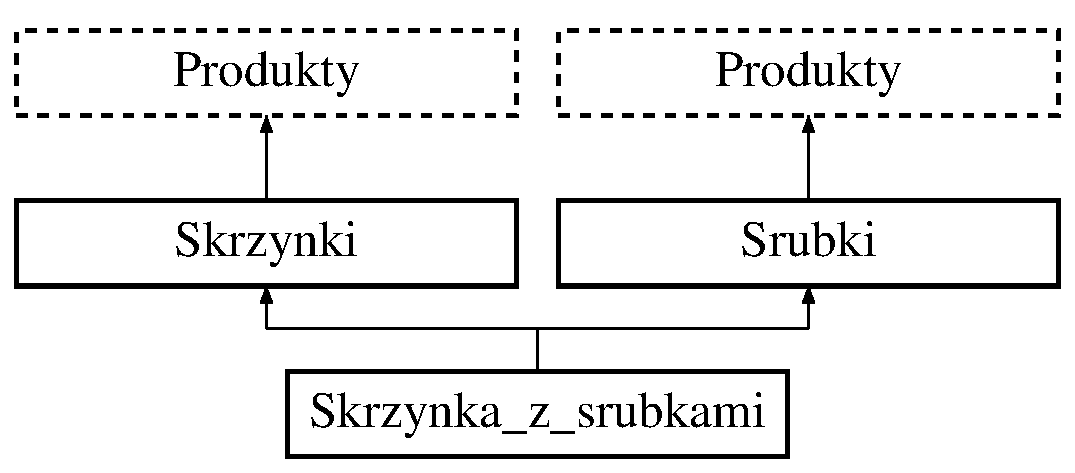
\includegraphics[height=3.000000cm]{class_skrzynka__z__srubkami}
\end{center}
\end{figure}
\subsection*{Public Member Functions}
\begin{DoxyCompactItemize}
\item 
void \mbox{\hyperlink{class_skrzynka__z__srubkami_a4726c1844080cb96e833cf16e977ecb3}{wstaw}} ()
\item 
void \mbox{\hyperlink{class_skrzynka__z__srubkami_ac543a438ce88bc79a9e8a398b6beff7c}{wypisz}} ()
\item 
void \mbox{\hyperlink{class_skrzynka__z__srubkami_a62ccdf02cb9d364630ebea27ea94f2a3}{zapisz}} (std\+::ostream \&o) const
\end{DoxyCompactItemize}
\subsection*{Additional Inherited Members}


\subsection{Detailed Description}
Klasa dziedziczaca po dwuch klasach nie abstrakcyjnych sluzaca do reprezentacji skrzynek z srobkami 

\subsection{Member Function Documentation}
\mbox{\Hypertarget{class_skrzynka__z__srubkami_a4726c1844080cb96e833cf16e977ecb3}\label{class_skrzynka__z__srubkami_a4726c1844080cb96e833cf16e977ecb3}} 
\index{Skrzynka\+\_\+z\+\_\+srubkami@{Skrzynka\+\_\+z\+\_\+srubkami}!wstaw@{wstaw}}
\index{wstaw@{wstaw}!Skrzynka\+\_\+z\+\_\+srubkami@{Skrzynka\+\_\+z\+\_\+srubkami}}
\subsubsection{\texorpdfstring{wstaw()}{wstaw()}}
{\footnotesize\ttfamily void Skrzynka\+\_\+z\+\_\+srubkami\+::wstaw (\begin{DoxyParamCaption}{ }\end{DoxyParamCaption})\hspace{0.3cm}{\ttfamily [virtual]}}

metoda sluzaca do wprowadzanaia danych charakteryzujacych skrzyneki z srobkami z klawiatury 

Reimplemented from \mbox{\hyperlink{class_skrzynki_a764d5064b25a294b3309dc5077a77921}{Skrzynki}}.

\mbox{\Hypertarget{class_skrzynka__z__srubkami_ac543a438ce88bc79a9e8a398b6beff7c}\label{class_skrzynka__z__srubkami_ac543a438ce88bc79a9e8a398b6beff7c}} 
\index{Skrzynka\+\_\+z\+\_\+srubkami@{Skrzynka\+\_\+z\+\_\+srubkami}!wypisz@{wypisz}}
\index{wypisz@{wypisz}!Skrzynka\+\_\+z\+\_\+srubkami@{Skrzynka\+\_\+z\+\_\+srubkami}}
\subsubsection{\texorpdfstring{wypisz()}{wypisz()}}
{\footnotesize\ttfamily void Skrzynka\+\_\+z\+\_\+srubkami\+::wypisz (\begin{DoxyParamCaption}{ }\end{DoxyParamCaption})\hspace{0.3cm}{\ttfamily [virtual]}}

metoda sluzaca do wypisywania danych charakteryzujacych skrzyneki z srobkami z klawiatury 

Reimplemented from \mbox{\hyperlink{class_skrzynki_adcf60a88ed78fba5a2dfdb54fa82b236}{Skrzynki}}.

\mbox{\Hypertarget{class_skrzynka__z__srubkami_a62ccdf02cb9d364630ebea27ea94f2a3}\label{class_skrzynka__z__srubkami_a62ccdf02cb9d364630ebea27ea94f2a3}} 
\index{Skrzynka\+\_\+z\+\_\+srubkami@{Skrzynka\+\_\+z\+\_\+srubkami}!zapisz@{zapisz}}
\index{zapisz@{zapisz}!Skrzynka\+\_\+z\+\_\+srubkami@{Skrzynka\+\_\+z\+\_\+srubkami}}
\subsubsection{\texorpdfstring{zapisz()}{zapisz()}}
{\footnotesize\ttfamily void Skrzynka\+\_\+z\+\_\+srubkami\+::zapisz (\begin{DoxyParamCaption}\item[{std\+::ostream \&}]{o }\end{DoxyParamCaption}) const\hspace{0.3cm}{\ttfamily [virtual]}}

metoda zapisujaca dane o skrzynekach z srobkami do pliku wprowadzane podczas dzialania programu 

Reimplemented from \mbox{\hyperlink{class_skrzynki_a2980647e51a17161872064efc5f1b185}{Skrzynki}}.



The documentation for this class was generated from the following files\+:\begin{DoxyCompactItemize}
\item 
Skrzynka\+\_\+z\+\_\+srubkami.\+h\item 
Skrzynka\+\_\+z\+\_\+srubkami.\+cpp\end{DoxyCompactItemize}

\hypertarget{class_skrzynki}{}\section{Skrzynki Class Reference}
\label{class_skrzynki}\index{Skrzynki@{Skrzynki}}


{\ttfamily \#include $<$Skrzynki.\+h$>$}

Inheritance diagram for Skrzynki\+:\begin{figure}[H]
\begin{center}
\leavevmode
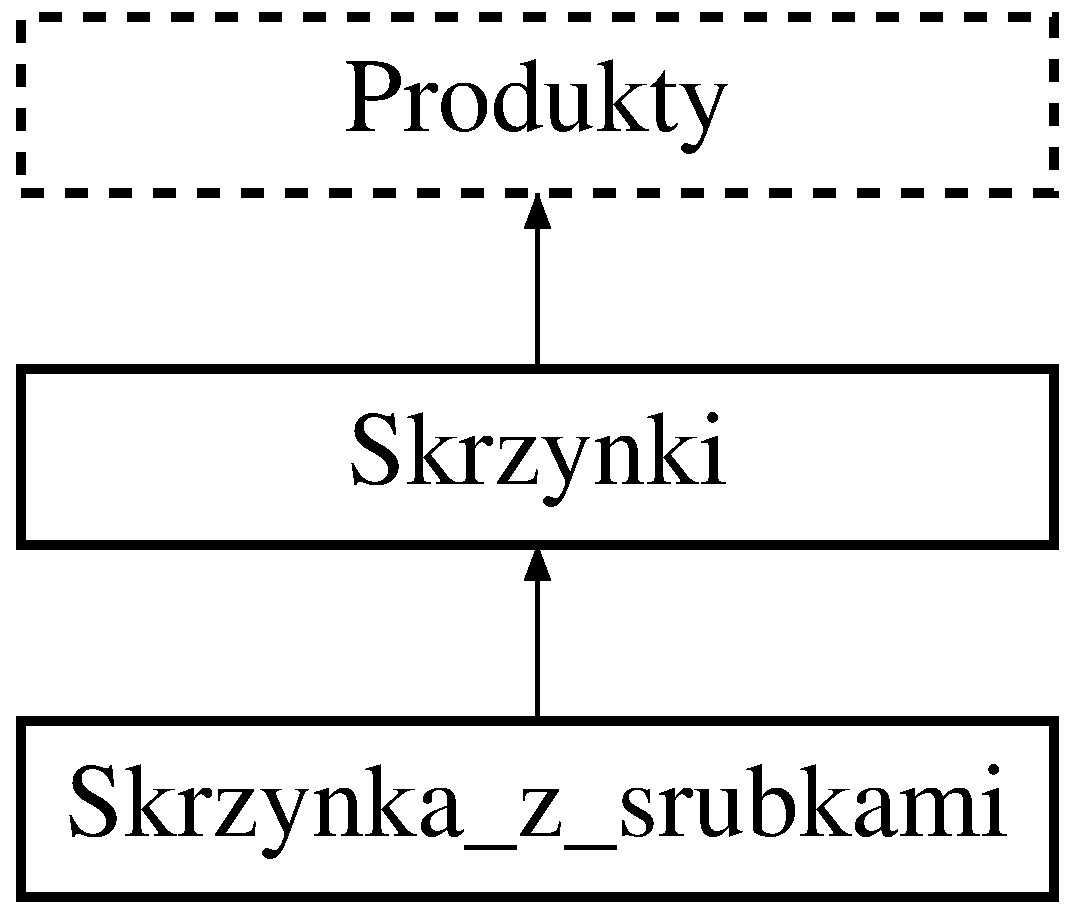
\includegraphics[height=3.000000cm]{class_skrzynki}
\end{center}
\end{figure}
\subsection*{Public Member Functions}
\begin{DoxyCompactItemize}
\item 
void \mbox{\hyperlink{class_skrzynki_a15e7e3b171152bd8e8a0fe5a72fcd249}{Wstaw\+\_\+ilosc}} ()
\item 
void \mbox{\hyperlink{class_skrzynki_aeb630b847e07d0b66a1ba76ff8bec293}{Wypisz\+\_\+ilosc}} ()
\item 
virtual void \mbox{\hyperlink{class_skrzynki_a764d5064b25a294b3309dc5077a77921}{wstaw}} ()
\item 
virtual void \mbox{\hyperlink{class_skrzynki_adcf60a88ed78fba5a2dfdb54fa82b236}{wypisz}} ()
\item 
virtual void \mbox{\hyperlink{class_skrzynki_a2980647e51a17161872064efc5f1b185}{zapisz}} (std\+::ostream \&o) const
\end{DoxyCompactItemize}
\subsection*{Protected Attributes}
\begin{DoxyCompactItemize}
\item 
\mbox{\Hypertarget{class_skrzynki_a93d76d16bac978c64614a03ccf621763}\label{class_skrzynki_a93d76d16bac978c64614a03ccf621763}} 
double {\bfseries ilosc}
\end{DoxyCompactItemize}
\subsection*{Additional Inherited Members}


\subsection{Detailed Description}
Klasa pochodna klasy produkty charakteryzujaca skrzynki 

\subsection{Member Function Documentation}
\mbox{\Hypertarget{class_skrzynki_a764d5064b25a294b3309dc5077a77921}\label{class_skrzynki_a764d5064b25a294b3309dc5077a77921}} 
\index{Skrzynki@{Skrzynki}!wstaw@{wstaw}}
\index{wstaw@{wstaw}!Skrzynki@{Skrzynki}}
\subsubsection{\texorpdfstring{wstaw()}{wstaw()}}
{\footnotesize\ttfamily void Skrzynki\+::wstaw (\begin{DoxyParamCaption}{ }\end{DoxyParamCaption})\hspace{0.3cm}{\ttfamily [virtual]}}

metoda sluzaca do wprowadzanaia danych charakteryzujacych skrzynki z klawiatury 

Reimplemented from \mbox{\hyperlink{class_produkty_ad69fa64c8984c55fe9b1a2ade607a0ed}{Produkty}}.



Reimplemented in \mbox{\hyperlink{class_skrzynka__z__srubkami_a4726c1844080cb96e833cf16e977ecb3}{Skrzynka\+\_\+z\+\_\+srubkami}}.

\mbox{\Hypertarget{class_skrzynki_a15e7e3b171152bd8e8a0fe5a72fcd249}\label{class_skrzynki_a15e7e3b171152bd8e8a0fe5a72fcd249}} 
\index{Skrzynki@{Skrzynki}!Wstaw\+\_\+ilosc@{Wstaw\+\_\+ilosc}}
\index{Wstaw\+\_\+ilosc@{Wstaw\+\_\+ilosc}!Skrzynki@{Skrzynki}}
\subsubsection{\texorpdfstring{Wstaw\+\_\+ilosc()}{Wstaw\_ilosc()}}
{\footnotesize\ttfamily void Skrzynki\+::\+Wstaw\+\_\+ilosc (\begin{DoxyParamCaption}{ }\end{DoxyParamCaption})}

metoda sluzaca do wprwadzania danych o ilosci miejsc w skrzynce, metode ta wykorzystuje funkcja wstaw \mbox{\Hypertarget{class_skrzynki_adcf60a88ed78fba5a2dfdb54fa82b236}\label{class_skrzynki_adcf60a88ed78fba5a2dfdb54fa82b236}} 
\index{Skrzynki@{Skrzynki}!wypisz@{wypisz}}
\index{wypisz@{wypisz}!Skrzynki@{Skrzynki}}
\subsubsection{\texorpdfstring{wypisz()}{wypisz()}}
{\footnotesize\ttfamily void Skrzynki\+::wypisz (\begin{DoxyParamCaption}{ }\end{DoxyParamCaption})\hspace{0.3cm}{\ttfamily [virtual]}}

metoda sluzaca do wypisywania danych charakteryzujacych skrzynki z klawiatury 

Reimplemented from \mbox{\hyperlink{class_produkty_a720c6591cfbb332f99baccf0f54c4ada}{Produkty}}.



Reimplemented in \mbox{\hyperlink{class_skrzynka__z__srubkami_ac543a438ce88bc79a9e8a398b6beff7c}{Skrzynka\+\_\+z\+\_\+srubkami}}.

\mbox{\Hypertarget{class_skrzynki_aeb630b847e07d0b66a1ba76ff8bec293}\label{class_skrzynki_aeb630b847e07d0b66a1ba76ff8bec293}} 
\index{Skrzynki@{Skrzynki}!Wypisz\+\_\+ilosc@{Wypisz\+\_\+ilosc}}
\index{Wypisz\+\_\+ilosc@{Wypisz\+\_\+ilosc}!Skrzynki@{Skrzynki}}
\subsubsection{\texorpdfstring{Wypisz\+\_\+ilosc()}{Wypisz\_ilosc()}}
{\footnotesize\ttfamily void Skrzynki\+::\+Wypisz\+\_\+ilosc (\begin{DoxyParamCaption}{ }\end{DoxyParamCaption})}

metoda sluzaca do wypisywania danych o ilosci miejsc w skrzynce, metode ta wykorzystuje funkcja wypisz \mbox{\Hypertarget{class_skrzynki_a2980647e51a17161872064efc5f1b185}\label{class_skrzynki_a2980647e51a17161872064efc5f1b185}} 
\index{Skrzynki@{Skrzynki}!zapisz@{zapisz}}
\index{zapisz@{zapisz}!Skrzynki@{Skrzynki}}
\subsubsection{\texorpdfstring{zapisz()}{zapisz()}}
{\footnotesize\ttfamily void Skrzynki\+::zapisz (\begin{DoxyParamCaption}\item[{std\+::ostream \&}]{o }\end{DoxyParamCaption}) const\hspace{0.3cm}{\ttfamily [virtual]}}

metoda zapisujaca dane o skrzynkach do pliku wprowadzane podczas dzialania programu 

Reimplemented from \mbox{\hyperlink{class_produkty_a49c2ba4084346df8e7c987b9ec62676e}{Produkty}}.



Reimplemented in \mbox{\hyperlink{class_skrzynka__z__srubkami_a62ccdf02cb9d364630ebea27ea94f2a3}{Skrzynka\+\_\+z\+\_\+srubkami}}.



The documentation for this class was generated from the following files\+:\begin{DoxyCompactItemize}
\item 
Skrzynki.\+h\item 
Skrzynki.\+cpp\end{DoxyCompactItemize}

\hypertarget{class_srubki}{}\section{Srubki Class Reference}
\label{class_srubki}\index{Srubki@{Srubki}}


{\ttfamily \#include $<$Srubki.\+h$>$}

Inheritance diagram for Srubki\+:\begin{figure}[H]
\begin{center}
\leavevmode
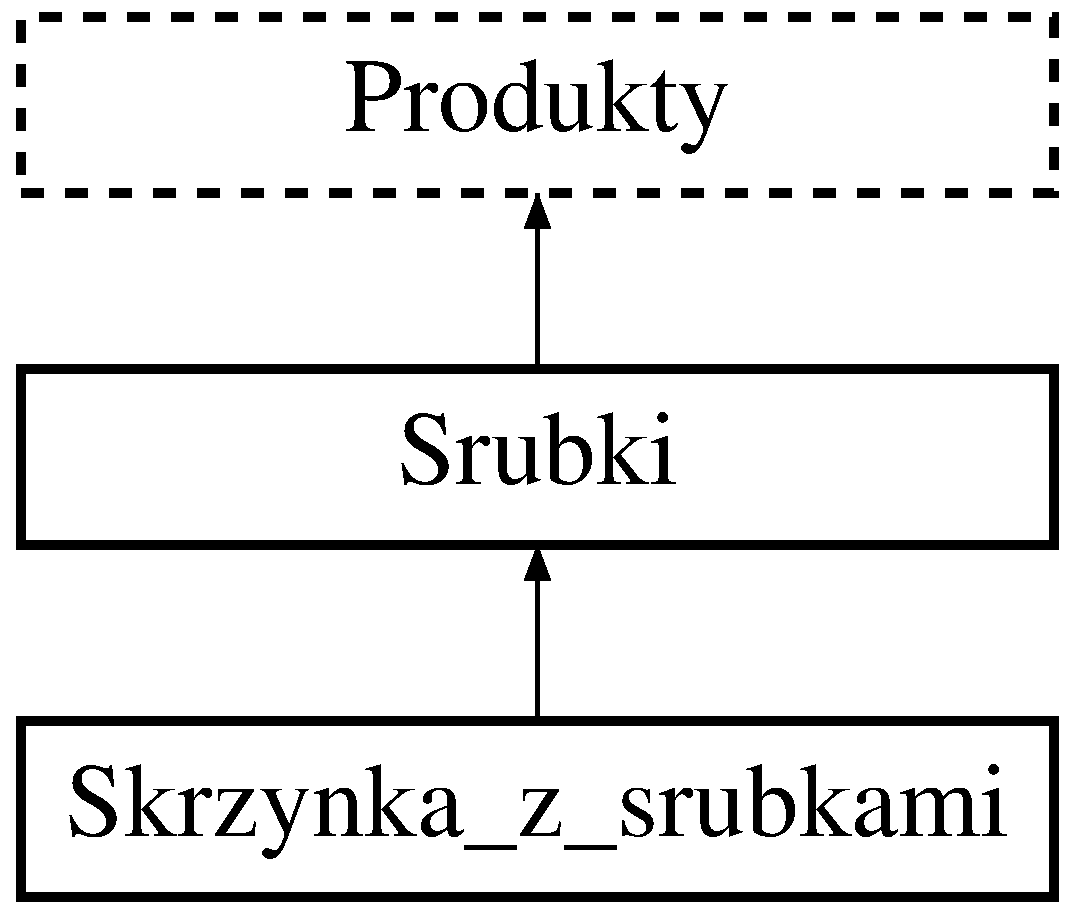
\includegraphics[height=3.000000cm]{class_srubki}
\end{center}
\end{figure}
\subsection*{Public Member Functions}
\begin{DoxyCompactItemize}
\item 
void \mbox{\hyperlink{class_srubki_a24162b0853a08261b4a48e9821a22478}{Wstaw\+\_\+waga}} ()
\item 
void \mbox{\hyperlink{class_srubki_a63a36d27654a13af2f8223ac28b3eae3}{Wypisz\+\_\+waga}} ()
\item 
virtual void \mbox{\hyperlink{class_srubki_a129b7fcf23ad1928f196ca255aa66438}{wstaw}} ()
\item 
virtual void \mbox{\hyperlink{class_srubki_a0ac1f1ce5748283a13b0f554add73f0b}{wypisz}} ()
\item 
virtual void \mbox{\hyperlink{class_srubki_a2d8edbd9d8170f12378c750f634a7ecd}{zapisz}} (std\+::ostream \&o) const
\end{DoxyCompactItemize}
\subsection*{Protected Attributes}
\begin{DoxyCompactItemize}
\item 
\mbox{\Hypertarget{class_srubki_aa9f5d21ee000de857932389c1919bb73}\label{class_srubki_aa9f5d21ee000de857932389c1919bb73}} 
float {\bfseries waga}
\end{DoxyCompactItemize}
\subsection*{Additional Inherited Members}


\subsection{Detailed Description}
Klasa dziedziczaca po klasie produkty umozliwia reprezentowanie danych o srobkach 

\subsection{Member Function Documentation}
\mbox{\Hypertarget{class_srubki_a129b7fcf23ad1928f196ca255aa66438}\label{class_srubki_a129b7fcf23ad1928f196ca255aa66438}} 
\index{Srubki@{Srubki}!wstaw@{wstaw}}
\index{wstaw@{wstaw}!Srubki@{Srubki}}
\subsubsection{\texorpdfstring{wstaw()}{wstaw()}}
{\footnotesize\ttfamily void Srubki\+::wstaw (\begin{DoxyParamCaption}{ }\end{DoxyParamCaption})\hspace{0.3cm}{\ttfamily [virtual]}}

metoda sluzaca do wprowadzanaia danych charakteryzujacych \mbox{\hyperlink{class_srubki}{Srubki}} z klawiatury 

Reimplemented from \mbox{\hyperlink{class_produkty_ad69fa64c8984c55fe9b1a2ade607a0ed}{Produkty}}.



Reimplemented in \mbox{\hyperlink{class_skrzynka__z__srubkami_a4726c1844080cb96e833cf16e977ecb3}{Skrzynka\+\_\+z\+\_\+srubkami}}.

\mbox{\Hypertarget{class_srubki_a24162b0853a08261b4a48e9821a22478}\label{class_srubki_a24162b0853a08261b4a48e9821a22478}} 
\index{Srubki@{Srubki}!Wstaw\+\_\+waga@{Wstaw\+\_\+waga}}
\index{Wstaw\+\_\+waga@{Wstaw\+\_\+waga}!Srubki@{Srubki}}
\subsubsection{\texorpdfstring{Wstaw\+\_\+waga()}{Wstaw\_waga()}}
{\footnotesize\ttfamily void Srubki\+::\+Wstaw\+\_\+waga (\begin{DoxyParamCaption}{ }\end{DoxyParamCaption})}

metoda sluzaca do wprwadzania danych o wadze, metode ta wykorzystuje funkcja wstaw \mbox{\Hypertarget{class_srubki_a0ac1f1ce5748283a13b0f554add73f0b}\label{class_srubki_a0ac1f1ce5748283a13b0f554add73f0b}} 
\index{Srubki@{Srubki}!wypisz@{wypisz}}
\index{wypisz@{wypisz}!Srubki@{Srubki}}
\subsubsection{\texorpdfstring{wypisz()}{wypisz()}}
{\footnotesize\ttfamily void Srubki\+::wypisz (\begin{DoxyParamCaption}{ }\end{DoxyParamCaption})\hspace{0.3cm}{\ttfamily [virtual]}}

metoda sluzaca do wypisywania danych charakteryzujacych \mbox{\hyperlink{class_srubki}{Srubki}} z klawiatury 

Reimplemented from \mbox{\hyperlink{class_produkty_a720c6591cfbb332f99baccf0f54c4ada}{Produkty}}.



Reimplemented in \mbox{\hyperlink{class_skrzynka__z__srubkami_ac543a438ce88bc79a9e8a398b6beff7c}{Skrzynka\+\_\+z\+\_\+srubkami}}.

\mbox{\Hypertarget{class_srubki_a63a36d27654a13af2f8223ac28b3eae3}\label{class_srubki_a63a36d27654a13af2f8223ac28b3eae3}} 
\index{Srubki@{Srubki}!Wypisz\+\_\+waga@{Wypisz\+\_\+waga}}
\index{Wypisz\+\_\+waga@{Wypisz\+\_\+waga}!Srubki@{Srubki}}
\subsubsection{\texorpdfstring{Wypisz\+\_\+waga()}{Wypisz\_waga()}}
{\footnotesize\ttfamily void Srubki\+::\+Wypisz\+\_\+waga (\begin{DoxyParamCaption}{ }\end{DoxyParamCaption})}

metoda sluzaca do wypisywania danych o wadze, metode ta wykorzystuje funkcja wypisz \mbox{\Hypertarget{class_srubki_a2d8edbd9d8170f12378c750f634a7ecd}\label{class_srubki_a2d8edbd9d8170f12378c750f634a7ecd}} 
\index{Srubki@{Srubki}!zapisz@{zapisz}}
\index{zapisz@{zapisz}!Srubki@{Srubki}}
\subsubsection{\texorpdfstring{zapisz()}{zapisz()}}
{\footnotesize\ttfamily void Srubki\+::zapisz (\begin{DoxyParamCaption}\item[{std\+::ostream \&}]{o }\end{DoxyParamCaption}) const\hspace{0.3cm}{\ttfamily [virtual]}}

metoda zapisujaca dane o srobkach do pliku wprowadzane podczas dzialania programu 

Reimplemented from \mbox{\hyperlink{class_produkty_a49c2ba4084346df8e7c987b9ec62676e}{Produkty}}.



Reimplemented in \mbox{\hyperlink{class_skrzynka__z__srubkami_a62ccdf02cb9d364630ebea27ea94f2a3}{Skrzynka\+\_\+z\+\_\+srubkami}}.



The documentation for this class was generated from the following files\+:\begin{DoxyCompactItemize}
\item 
Srubki.\+h\item 
Srubki.\+cpp\end{DoxyCompactItemize}

%--- End generated contents ---

% Index
\backmatter
\newpage
\phantomsection
\clearemptydoublepage
\addcontentsline{toc}{chapter}{Index}
\printindex

\end{document}
